% 1. Стиль и язык
\documentclass[utf8x, 14pt]{G7-32} % Стиль (по умолчанию будет 14pt)
% Остальные стандартные настройки убраны в preamble.inc.tex.
\sloppy

% Настройки стиля ГОСТ 7-32
% Для начала определяем, хотим мы или нет, чтобы рисунки и таблицы нумеровались в пределах раздела, или нам нужна сквозная нумерация.
\EqInChapter % формулы будут нумероваться в пределах раздела
\TableInChapter % таблицы будут нумероваться в пределах раздела
\PicInChapter % рисунки будут нумероваться в пределах раздела

% Добавляем гипертекстовое оглавление в PDF
\usepackage[
bookmarks=true, colorlinks=true, unicode=true,
urlcolor=black,linkcolor=black, anchorcolor=black,
citecolor=black, menucolor=black, filecolor=black,
]{hyperref}

\AfterHyperrefFix

\usepackage{microtype}% полезный пакет для микротипографии, увы под xelatex мало чего умеет, но под pdflatex хорошо улучшает читаемость

% Тире могут быть невидимы в Adobe Reader
\ifInvisibleDashes
\MakeDashesBold
\fi

\usepackage{graphicx}   % Пакет для включения рисунков

% С такими оно полями оно работает по-умолчанию:
% \RequirePackage[left=20mm,right=10mm,top=20mm,bottom=20mm,headsep=0pt,includefoot]{geometry}
% Если вас тошнит от поля в 10мм --- увеличивайте до 20-ти, ну и про переплёт не забывайте:
\geometry{right=20mm}
\geometry{left=30mm}
\geometry{bottom=20mm}
\geometry{ignorefoot}% считать от нижней границы текста


% Пакет Tikz
\usepackage{tikz}
\usetikzlibrary{arrows,positioning,shadows}

% Произвольная нумерация списков.
\usepackage{enumerate}

% ячейки в несколько строчек
\usepackage{multirow}

% itemize внутри tabular
\usepackage{paralist,array}

%\setlength{\parskip}{1ex plus0.5ex minus0.5ex} % разрыв между абзацами
\setlength{\parskip}{1ex} % разрыв между абзацами
\usepackage{blindtext}

% Центрирование подписей к плавающим окружениям
%\usepackage[justification=centering]{caption}
\usepackage{newfloat}

% Алгоритмы
\usepackage[ruled,vlined]{algorithm2e}
\SetAlgorithmName{Алгоритм}{алгоритм}{Список алгоритмов}

% Математика
\usepackage{amsmath}

% Код
\usepackage{courier}
\usepackage{listings}             % Include the listings-package

% Изображения
% \usepackage[demo]{graphicx}
% \usepackage{caption}
\usepackage{subcaption}
\graphicspath{ {Pictures/} }

\DeclareFloatingEnvironment[
placement={!ht},
name=Equation
]{eqndescNoIndent}
\edef\fixEqndesc{\noexpand\setlength{\noexpand\parindent}{\the\parindent}\noexpand\setlength{\noexpand\parskip}{\the\parskip}}
\newenvironment{eqndesc}[1][!ht]{%
    \begin{eqndescNoIndent}[#1]%
\fixEqndesc%
}
{\end{eqndescNoIndent}}
\setcounter{page}{5}
\setmainfont{Times New Roman}
\setlength{\parskip}{0em}
% Настройки листингов.
% \ifPDFTeX
% 8 Листинги

\usepackage{listings}

% Значения по умолчанию
\lstset{
  keepspaces=true,
  basicstyle= \footnotesize\ttfamily,
  breakatwhitespace=true,% разрыв строк только на whitespacce
  breaklines=true,       % переносить длинные строки
%   captionpos=b,          % подписи снизу -- вроде не надо
  inputencoding=koi8-r,
  numbers=left,          % нумерация слева
  numberstyle=\footnotesize,
  showspaces=false,      % показывать пробелы подчеркиваниями -- идиотизм 70-х годов
  showstringspaces=false,
  showtabs=false,        % и табы тоже
  stepnumber=1,
  tabsize=4,              % кому нужны табы по 8 символов?
  frame=single
}

% Стиль для псевдокода: строчки обычно короткие, поэтому размер шрифта побольше
\lstdefinestyle{pseudocode}{
  basicstyle=\small,
  keywordstyle=\color{black}\bfseries\underbar,
  language=Pseudocode,
  numberstyle=\footnotesize,
  commentstyle=\footnotesize\it
}

% Стиль для обычного кода: маленький шрифт
\lstdefinestyle{realcode}{
  basicstyle=\scriptsize,
  numberstyle=\footnotesize
}

% Стиль для коротких кусков обычного кода: средний шрифт
\lstdefinestyle{simplecode}{
  basicstyle=\footnotesize,
  numberstyle=\footnotesize
}

% Стиль для BNF
\lstdefinestyle{grammar}{
  basicstyle=\footnotesize,
  numberstyle=\footnotesize,
  stringstyle=\bfseries\ttfamily,
  language=BNF
}

% Определим свой язык для написания псевдокодов на основе Python
\lstdefinelanguage[]{Pseudocode}[]{Python}{
  morekeywords={each,empty,wait,do},% ключевые слова добавлять сюда
  morecomment=[s]{\{}{\}},% комменты {а-ля Pascal} смотрятся нагляднее
  literate=% а сюда добавлять операторы, которые хотите отображать как мат. символы
    {->}{\ensuremath{$\rightarrow$}~}2%
    {<-}{\ensuremath{$\leftarrow$}~}2%
    {:=}{\ensuremath{$\leftarrow$}~}2%
    {<--}{\ensuremath{$\Longleftarrow$}~}2%
}[keywords,comments]

% Свой язык для задания грамматик в BNF
\lstdefinelanguage[]{BNF}[]{}{
  morekeywords={},
  morecomment=[s]{@}{@},
  morestring=[b]",%
  literate=%
    {->}{\ensuremath{$\rightarrow$}~}2%
    {*}{\ensuremath{$^*$}~}2%
    {+}{\ensuremath{$^+$}~}2%
    {|}{\ensuremath{$|$}~}2%
}[keywords,comments,strings]

% Подписи к листингам на русском языке.
\renewcommand\lstlistingname{Листинг}
\renewcommand\lstlistlistingname{Листинги}

% \else
% \usepackage{local-minted}
% \fi

% Полезные макросы листингов.
% Любимые команды
\newcommand{\Code}[1]{\textbf{#1}}


\begin{document}

\frontmatter % выключает нумерацию ВСЕГО; здесь начинаются ненумерованные главы: реферат, введение, глоссарий, сокращения и прочее.


%\listoffigures                         % Список рисунков

%\listoftables                          % Список таблиц

%\NormRefs % Нормативные ссылки 
% Команды \breakingbeforechapters и \nonbreakingbeforechapters
% управляют разрывом страницы перед главами.
% По-умолчанию страница разрывается.

% \nobreakingbeforechapters
% \breakingbeforechapters

\tableofcontents

% \printnomenclature % Автоматический список сокращений

\Introduction
Стеганография --- это практика сокрытия сообщения внутри другого сообщения или физического объекта.
Тогда как криптография скрывает содержимое сообщение, стеганография скрывает сам факт существования какого-либо сообщения. 

Стеганография часто используется совместно с криптографией, дополняя ее.
Стеганографические методы сокрытия сообщения снижают вероятность обнаружения самой передачи сообщения.
Если сообщение к тому же зашифровано, то это обеспечивает еще большую защищенность. 

В настоящее время наибольшее распространение получила цифровая стеганография.
Особенностью цифровой стеганографии является сокрытие информации внутри других цифровых объектов,
таких как текст, изображения, видео, аудио и другие.
Со все большим возрастанием роли интернет-технологий в жизни человека значимость стеганографии также возрастает.

Области применения стеганографии включают в себя:
\begin{enumerate}
    \item Защита авторского права и DRM (digital rights management).
    \item Незаметная передача информации.
    \item Защита конфиденциальной информации от несанкционированного доступа.
\end{enumerate}

Цифровая стеганография является молодым и бурно развивающимся направлением.
Несмотря на свою востребованность, стеганография очень слабо освещается в программах обучения информационной безопасности.
Моя работа призвана восполнить этот пробел.

В своей работе я хочу рассмотреть основные стеганографические алгоритмы, определить области их применения,
достоинства и недостатки, а также провести анализ возможных уязвимостей этих алгоритмов.


\mainmatter % это включает нумерацию глав и секций в документе ниже

\chapter{Теоретические аспекты изучаемой темы}

\section{Основные понятия}

\begin{enumerate}
    \item Стеганографическая система (стегосистема) --- совокупность методов и средств,
    используемых для создания скрытого канала для передачи информации.
    Основные требования, предъявляемые к стегосистеме:
    \begin{enumerate}
        \item Безопасность системы определяется секретностью ключа.
        Это означает, что даже если потенциальный враг представляет работу стеганографической системы
        и статистические характеристики сообщений и контейнеров,
        это не дает ему дополнительных преимуществ при выявлении
        наличия или отсутствия сообщения в конкретном контейнере.
        \item При обнаружении противником наличия скрытого сообщения
        он не должен смочь извлечь сообщение до тех пор, пока он не будет владеть ключом.
        \item Алгоритм сокрытия информации не нарушает ее целостность и аутентичность.
        В некоторых случаях дополнительно требуется,
        чтобы алгоритм обеспечивал целостность сообщения при деформации контейнера.
        \item Система с цифровым водяным знаком должна иметь низкую вероятность ложного обнаружения скрытого сообщения.
    \end{enumerate}
    \item Сообщение --- информация, передачу которой нужно скрыть.
    \item Контейнер --- любая информация,
    используемая для сокрытия тайного сообщения. Контейнер может находиться в одном из двух состояний:
    \begin{enumerate}
        \item Пустой контейнер --- контейнер, не содержащий сообщение.
        \item Заполненный контейнер (стегоконтейнер) --- контейнер, содержащий сообщение.
    \end{enumerate}
    \item Стеганографический канал (стегоканал) --- канал передачи стегоконтейнера.
    \item Ключ (стегоключ) --- секретный ключ, нужный для сокрытия стегоконтейнера.
    По аналогии с криптографией стегоключи подразделяются на 2 типа:
    \begin{enumerate}
        \item Закрытый стегоключ.
        В системах с закрытым стегоключем ключ должен быть создан до начала обмена сообщениями,
        либо передан по защищенному каналу связи.
        \item Открытый стегоключ. Такой ключ может быть передан по открытому незащищенному каналу связи.
        Открытый стегоключ должен обладать таким свойством, чтобы по нему вычислительно нецелесообразно
        было восстанавливать закрытый ключ.
    \end{enumerate}
\end{enumerate}

\section{Цифровые водяные знаки и цифровые отпечатки}

Цифровой водяной знак (ЦВЗ) --- технология, созданная для защиты авторский прав на цифровые объекты.
В связи с быстрым развитием информационных технологий все более актуальным становится
вопрос защиты авторских прав и интеллектуальной собственности, представленной в цифровом виде.
Примерами цифровых объектов могут выступать аудиозаписи, видеозаписи, изображения, электронные книги и другие. 
ЦВЗ могут быть как видимыми, так и невидимыми. Решение о наличии в цифровом объекте невидимого ЦВЗ принимаются
на основе процедуры декодирования.

В общем виде стегосистема ЦВЗ может быть разбита на части следующим образом:
\begin{enumerate}
    \item Прекодер --- часть, которая приводит ЦВЗ к удобному для встраивания в стегоконтейнер виду.
    \item Стегокодер --- часть, которая вкладывает сообщение в стегоконтейнер.
    \item Выделение встроенного сообщения --- процедура, выделяющие сообщение из стегоконтейнера.
    \item Стегодетектор --- часть, определяющая наличие ЦВЗ.
    \item Декодер --- часть, восстанавливающая исходное сообщение.
\end{enumerate}

Контейнер, содержащий ЦВЗ, может подвергаться преднамеренным атакам или случайным помехам.
Стегосистема ЦВЗ должна обеспечивать как различимость самого стегоконтейнера человеком,
потому как в качестве стегоконтейнера выступает интеллектуальная собственность,
нацеленная на конечного потребителя, так и различимость ЦВЗ стегодетектором,
который может подтвердить или опровергнуть авторские права на интеллектуальную собственность.
В связи с этим в стегосистемах ЦВЗ применяется помехоустойчивое кодирование и метод широкополосного сигнала.

Одной из основных характеристик ЦВЗ является надежность.
Под надежность понимается устойчивость к различным деформациям контейнера.
По отношению к этой характеристика ЦВЗ распадается на три класса:
\begin{enumerate}
    \item Хрупкие.
    Такие ЦВЗ разрушается при небольших модификациях заполненного стегоконтейнера.
    Такие ЦВЗ применяются для аутентификации сигнала.
    Например, такие ЦВЗ используются для подтверждения подлинности цифрового объекта.
    \item Полухрупкие.
    Такие ЦВЗ чувствительны к некоторым преобразованиям контейнера и нечувствительны к другим.
    Например, ЦВЗ, встроенное в изображение, может быть нечувствительно к его компрессии,
    но в то же время быть чувствительно к вырезке из этого изображения фрагмента.
    \item Робастные или надежные.
    Такие ЦВЗ устойчивы к разным видам воздействия на контейнер.
    Такие ЦВЗ часто применяются при защите от копирования.
\end{enumerate}

Похожим на ЦВЗ, но отличающимся понятием является цифровой отпечаток.
ЦВЗ предполагает встраивание одного и того же сообщения в различные контейнеры.
В случае же цифрового отпечатка в каждый контейнер встраивается уникальное сообщение.
Часто областью применения цифровых отпечатков становится защита исключительного права.
В качестве сообщения в таком случае встраивается информация, указывающая на идентифицирующие данные покупателя.
Эти данные позволят отследить источник распространения, если произойдет утечка стегоконтейнера.

\section{Обобщенные стеганографические методы}
К настоящему моменту разработано множество стеганографических методов скрытия информации.
Для их систематичного изучения удобно группировать их по схожим признакам.
\begin{enumerate}
    \item Пространственные методы. Особенностью этих методов является сокрытие информации напрямую
    в пространственной области контейнера. Например,
    в случае звукового контейнера  таким пространством могут быть семплы,
    а в случае изображения --- пиксели.
    \item Частотные методы. Такие методы сначала используют одно из интегральный преобразований сигнала,
    чтобы перейти в его частотную область. Далее кодирование сообщение производится за счет изменения частотных
    характеристик сигнала. После этого используется обратное преобразование, чтобы получить модифицированный сигнал,
    содержащий закодированное сообщение.
    \item Алгоритмы, использующие особенности формата файла. Такие алгоритмы как правило записывают
    сообщение в метаданные файла или в иные неиспользуемые поля файла.
\end{enumerate}

\section{Стегоанализ}
Стегоанализ --- это наука о выявлении сообщений, скрытых методами стеганографии.
Задача стегоанализа --- выявить подозрительные контейнеры, определить, есть ли в них скрытое сообщение,
и, если возможно, восстановить это сообщение.

Если в случае криптоанализа аналитик начинает работу сразу с зашифрованным сообщением,
то в случае стегоанализа аналитик начинает работу с множества подозрительных файлов,
о которых как правило мало что известно. Деятельность аналитика в таком случае
начинается с сокращения этого множества файлов до подмножества, в котором файлы
скорее всего были заполнены сообщением.

Основной техникой, используемой в стегоанализе, является статистический анализ.
Сначала множество незаполненных контейнеров одного типа анализируется для получения
различной статистики. Затем эта статистка используется при классификации контейнера
как заполненного или пустого. При такой классификации могут быть использованы
самые различные наблюдения:
\begin{enumerate}
    \item Сокрытие информации может приводить к изменению статистической структуры
    контейнера, в результате чего соседние элементы контейнера становятся попарно ближе
    друг к другу. На этом основана атака хи-квадрат.
    \item Сокрытие информации увеличивает энтропию контейнера. В результате чего он
    хуже поддается сжатию. На этом основана атака с помощью алгоритмов сжатия.
\end{enumerate}
Так же для такой классификации могут быть использованы методы машинного обучения.
\chapter{LSB}
\section{Общие сведения}
LSB (least significant bit) --- стеганографический метод сокрытия информации, основанный на замене поседних значащих бит
элементов контейнера битами сообщения. Этот метод использует тот факт,
что уровень детализации во многих контейнерах гораздо выше того,
что может воспринять и различить человек.
Следовательно, заполенный контейнер будет неотличим от оригинального
для человеческого восприятия. В качестве примера можно взять
полутоновое изображение с градациями серого. Цвет кодируется одним байтом.
Человеческий глаз воспринимает только первые 7 байт,
а самый младший бит вносит там мало информации, что человек не сможет заметить разницу.

LSB обладает следующими достоинствами:
\begin{enumerate}
    \item Простота реализации и эффективность.
    \item Низкая вычислительная сложность.
    \item Пустой и заполненный контейнер неразличимы для органов восприятия человека
\end{enumerate}
И недостатками:
\begin{enumerate}
    \item Метод применим лишь к контейнерам, которые хранят данные без сжатия или используют
    сжатие без потерь, так как информации, закодированная в наименее значимых битах, может
    быть потеряна в процессе сжатия.
    \item Небольшие трансформации контейнера приводят к невозможности восстановить сообщение.
    Например, если сообщение скрыто в изображении методом LSB, то небольшие линейные трансформации
    (вращение, движение, отражение, гомотетия, сжатие, растяжение) уничтожат сообщение. Так же
    сообщение разрушается в результате сжатия с потерями. Все это говорит о том, что метод обладает
    низкой робастостью.
    \item Факт сокрытия изображения легко обнаруживает методами стегоанализа.
\end{enumerate}

Ввиду перечисленных выше недостатков очевидным кажется недопустимость использования
данного методы для сокрытия ЦВЗ.

\section{Алгоритм}
Перейдем к конкретным реализациям этого метода. Алгоритм~\ref{alg:lsb_encode}
демонстрирует псевдокод сокрытия методом LSB.
\begin{algorithm}[ht!]
    \KwData{Контейнер, Сообщение}
    \KwResult{Заполненный стегоконтейнер}
     $N \leftarrow$ Длина сообщения в битах\;
     $Message \leftarrow$ Бинарное представление сообщения\;
     $Container \leftarrow$ Массив с элементами контейнера\;
     \For{$i = 1, 2, \ldots, N$}{
         \eIf{$Container[i] \equiv Message[i] \pmod{2}$}{
             \textbf{continue\;}
         }{
             $Container[i] \leftarrow (Container[i] \land \neg 1) \lor Message[i]$\;
         }
     }
     \caption{LSB Кодирование}
    \label{alg:lsb_encode}
\end{algorithm}
\begin{algorithm}[ht!]
    \KwData{Заполненный контейнер}
    \KwResult{Сообщение в бинарном представлении}
    $Message \leftarrow$ Пустой список\;
    $Container \leftarrow$ Массив с элементами контнейнера\;
    $N \leftarrow$ Длина $Container$\;
    \For{$i = 1, 2, \ldots, N$}{
        \eIf{$Container[i] \equiv 0 \pmod{2}$}{
            $Message.append(0)$\;
        }{
            $Message.append(1)$\;
        }
    }
    \caption{LSB Декодирование}
    \label{alg:lsb_decode}
\end{algorithm}

Как видно, сначала сообщение преобразуется в бинарный вид,
а затем кодируется в элементах контейнера за счет изменения четности младшего бита.
Логические операции в данном случае соответствуют бинарным операциям на компьютере.
В итоге последние биты элементов контейнера в точности повторяют сообщение.
Так же можно заметить, что единственная часть алгоритма, зависящая от контейнера
--- это выделение массива элементов из контейнера. Алгоритм~\ref{alg:lsb_decode}
показывает, как декодировать сообщение из заполненного стегоконтейнера.

Реализуем этот алгоритм в виде класса на Python. Как уже было сказано,
существенная часть алгоритма не зависит от контейнера,
поэтому целесообразно реализовать алгоритм как абстрактный класс,
от которого будут наследоваться реализации для конкретных контейнеров.
\lstinputlisting[language=Python, style=simplecode, caption=Абстрактный класс LSB, frame=single]{Code/lsb.py}

Как видно, в методах нет циклов \textbf{for}. Они скрыты за интерфейсом библиотеки numpy.
Интерфейс библиотеки numpy позволяет нам применят операции к матрицам,
из-за чего код выглядет лаконичнее. К тому же библиотека написана на языке C,
поэтому ее код работает очень быстро.

Напишем реализацию LSB для PNG. Прежде чем реализовать метод LSB для PNG-контейнера,
имеет смысл коротко изложить формат данных PNG.

\section{Формат файла PNG}

В самом общем виде PNG файл представляет из себя сигнатуру,
за которой следует последовательность блоков,
как показано на рисунке~\ref{img:png_1}
\begin{figure}[ht!]
    \caption{Общий вид формата PNG}
    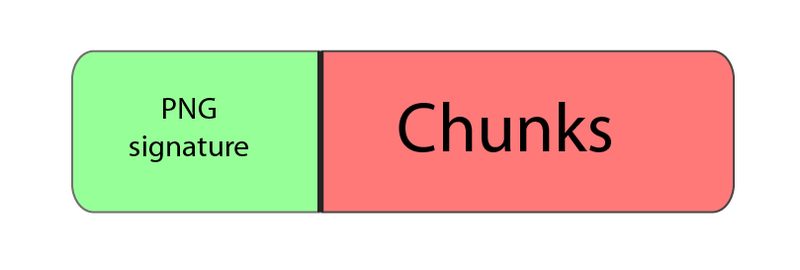
\includegraphics{PNG/1}
    \centering
    \label{img:png_1}
\end{figure}

Сигнатура PNG файла состоит из 8 байт, в hex нотации они выглядят так:
\textbf{89 50 4E 47 0D 0A 1A 0A}.

Каждый блок состоит из четырех секций: длина, тип, содержание, CRC, --- как показано на рисунке~\ref{img:png_2}:
\begin{figure}[ht!]
    \caption{Общий вид чанка}
    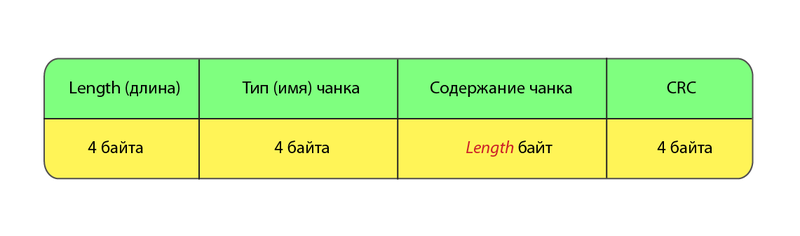
\includegraphics{PNG/2}
    \centering
    \label{img:png_2}
\end{figure}
В длине указывается длина блока в байтах. Тип указывается с помощью четырех ascii символов,
чувствительных к регистру. С помощью регистра декодеру передает дополнительная информация, а именно:
\begin{enumerate}
    \item Регистр первого символа сообщает, является данный блок критическим или нет. Критические
    блоки распознаются каждым декодером. Если декодер не может распознать тип такого блока,
    он аварийно завершает работу.
    \item Регистр второго символа задает публичность или приватность блока.
    Публичные блоки обычно официальные и хорошо задокументированы. Чтобы закодировать в библиотека
    какую-то специфичную информацию, его тип можно изменить на приватный.
    \item Регистр третьего символа зарезервирован на будущее. По умолчанию там стоит символ в большом регистре.
    \item Регистр четвертого символа сообщает возможность копирования данного блока редакторами.
\end{enumerate}

Список критических блоков:
\begin{enumerate}
    \item IHDR --- заголовочный блок, содержающий основную информацию об изображении.
    \item PLTE --- палитра изображения.
    \item IDAT --- содержит непосредственно изображение.
    В любом PNG файле должно быть не менее одного такого блока.
    \item IEND --- завершающих чанк. Должен находиться в самом конце файла.
\end{enumerate}

Список некритических блоков:
\begin{enumerate}
    \item bKGD --- блок, задающий фоновый цвет изображения.
    \item cHRM --- блок, используемый для задания цветового пространства CIE 1931.
    \item gAMA --- определяет гамму.
    \item hIST --- хранит гистограмму изображения либо общее содержания каждого цвета в рисунке.
    \item iTXt --- содержит текст в UTF-8
    \item pHYs --- содержит размер пикселя или отношение сторон изобарежния.
    \item sRGB --- свидетельствует об использовании sRGM схемы.
    \item tIME --- дата последнего изменения изображения.
    \item tRNS --- информация о прозрачности.
\end{enumerate}

Согласно вышесказанному, минимальный PNG файл выглядит так,
как показано на рисунке~\ref{img:png_3}

\begin{figure}[ht!]
    \caption{Минимальный PNG}
    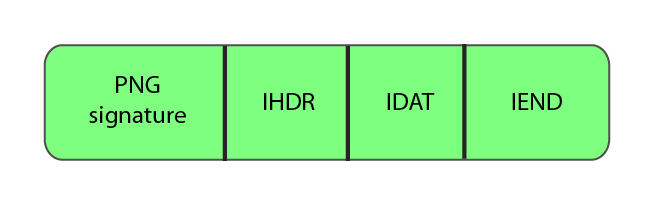
\includegraphics{PNG/3}
    \centering
    \label{img:png_3}
\end{figure}

В следующей секции представлены данные блока.
В секции CRC записан CRC блока.

Наиболее интересными для нас являются блоки с типами IHDR и IDAT.
IHDR --- заголовочный блок, который является обязательным для PNG файла.
Он содержит следующие интересующие нас поля:
\begin{enumerate}
    \item Ширина изображения в пикселях.
    \item Высота изображения в пикселях.
    \item Битовая глубина, задающее количество бит на каждый сэмпл.
    \item Тип цвета. Возможны следующие значения:
    \begin{enumerate}
        \item Градация серого
        \item RGB
        \item Индексы из палитры
        \item Градация серого и альфа-канал
        \item RGB и альфа-канал
    \end{enumerate}
\end{enumerate}

Блок IDAT содержит сжатые данные изображения.
На данный момент поддерживается только сжатия по алгоритму deflate.

\section{Реализация LSB для контейнера PNG}
PNG изображение представимо в виде матрицы, элементами которой являются пиксели.
В случае RGB каждый пиксель представляет элементы из трех каналов, каждый из каналов
в отдельности может рассматриваться как градация серого. В случае градации серого каждый
пиксель просто представлен значением от 0 до 255.
Чтобы закодировать сообщение в эту матрицу, склеим ее строки друг с другом в одну большую строку,
равно как и склеим каналы, чтобы они образовали последовательность элементов.
Именно это делает метод \textbf{\_ to \_ elements}.
Такой метод одинаково хорошо подходит и для разных типов цвета: RGB, RGB и альфа-канала,
градации серого, градации серого и альфа-канала.
Чтобы из элементов получить двумерную RGB матрицу,
проделаем обратную операцию, что и далет метод \textbf{\_ from \_ elements}.

В функции \textbf{main} используем как сообщение книгу "Алиса в стране чудес" в оригинале.
Считаем файл с книгой как последовательность байт и закодируем в изображение с помощью LSB.
Далее выполним декодирование и сверим полученные данные.
Исходный код представлен в листинге~\ref{code:png}.
\lstinputlisting[language=Python, label={code:png}, style=simplecode, caption=реализация LSB для PNG, frame=single]{Code/png.py}
Сравнение изображение до и после заполнения контейнера методом LSB
привидено на рисунке~\ref{img:lsb}.
Как видно, два рисунка визуально неотличимы,
хотя в одном из них закодировано 150 килобайт информации.
\begin{figure}[ht!]
    \centering
    \begin{subfigure}{.5\textwidth}
      \centering
      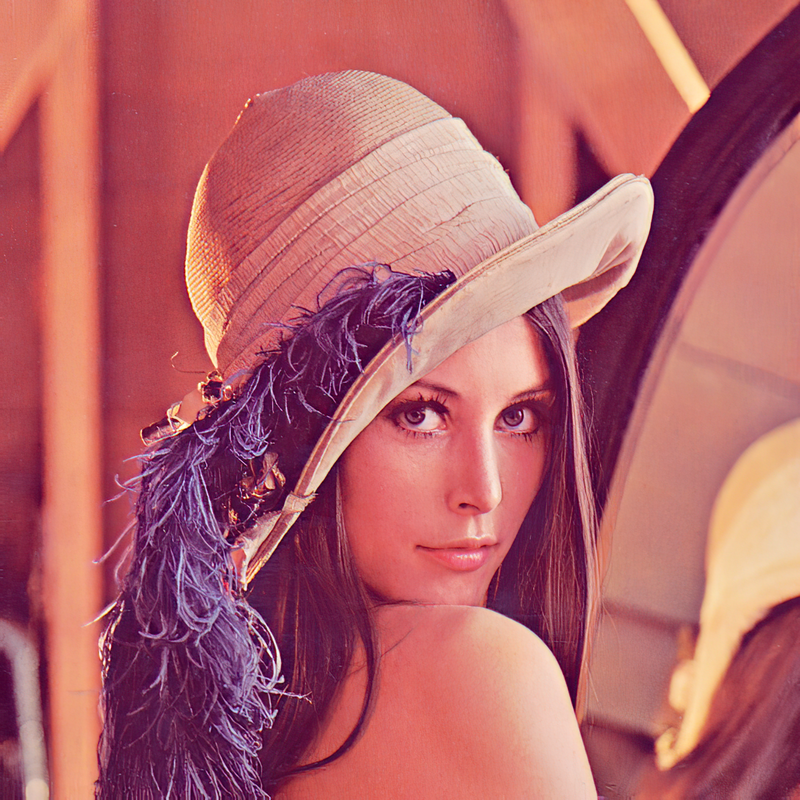
\includegraphics[width=.9\linewidth]{PNG/Lenna.png}
      \caption{Оригинал}
      \label{img:lenna-png}
    \end{subfigure}%
    \begin{subfigure}{.5\textwidth}
      \centering
      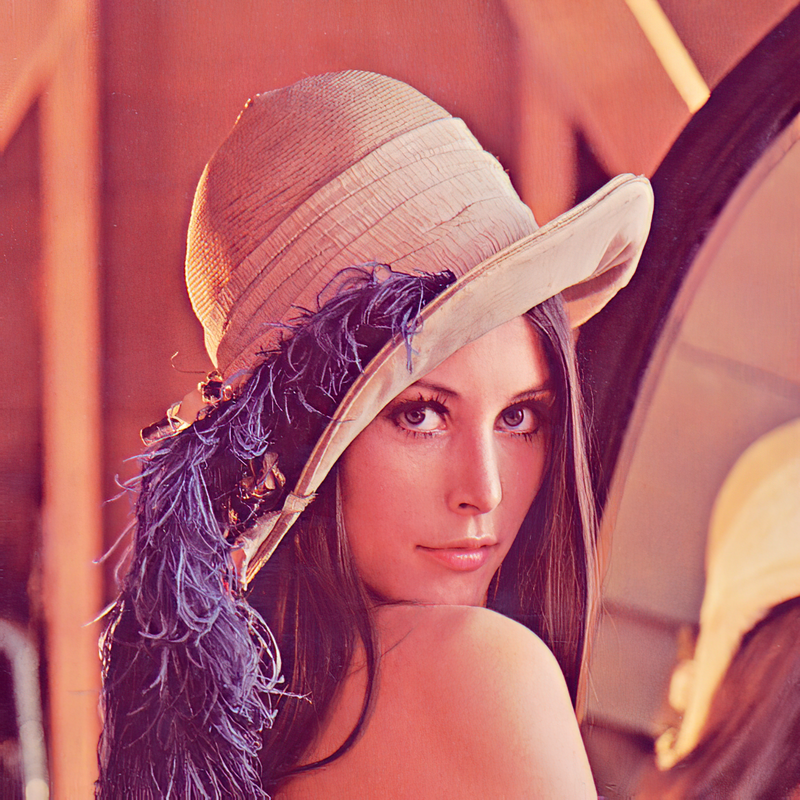
\includegraphics[width=.9\linewidth]{PNG/LSB_Lenna.png}
      \caption{После приминения LSB}
      \label{img:lenna-lsb}
    \end{subfigure}
    \caption{Изображение до и после приминения LSB}
    \label{img:lsb}
\end{figure}
\chapter{Сокрытие в спектральной области}
\section{Дискретное косинусное преобразование}
Дискретное косинусное преобразование (ДКП) --- одно из дискретных преобразований Фурье.
ДКП представляет конечную последовательность в виде суммы функций косинуса,
колеблющихся на разных частотах. ДКП широко используется при обработке сигналов и сжатии данных.
Например, ДКП используется при сжатии в изображениях (JPEG, HEIF), аудиофайлах (Dolby Digital, MP3),
видеофайлах (MPEG, H.26x), в цифровом телевидении (SDTV, HDTV, VOD) и в других.

ДКП является линейным ортогональным преобразованием. Как любое дискретное линейное преобразование,
ДКП можно представить в виде матрицы. Будучи ортоганальным преобразованием, обратное к ДКП преобразование
задает транспонированной матрицей ДКП, домноженной на какой-то коэффициент.

Использование косинусных, а не синусоидальных функций имеет решающее значение для сжатия,
поскольку для аппроксимации типичного сигнала требуется меньше косинусных функций.
ДКП подобно дискретному преобразованию Фурье, но использующее только действительные числа.

Существует 8 стандартных типов ДКП, однако наиболее употребимым является второй тип,
который часто называют просто ДКП (DCT-II).
Формула дискретного косинусного преобразования выглядит так,
как показано в формуле~\ref{eq:simple-dcp}:
\begin{equation} \label{eq:simple-dcp}
    X_k = \sum_{n=0}^{N-1} x_n \cos \left[\frac{\pi}{N} \left(n+\frac{1}{2}\right) k \right] \quad \quad k = 0, \dots, N-1    
\end{equation}
Формула для матрицы преобразования выглядит как формуле~\ref{eq:matrix-dcp}:
\begin{equation} \label{eq:matrix-dcp}
    {DCT}\text{-}2_n= \left[\cos (k(l+\tfrac{1}{2})\tfrac{\pi}{n})\right]_{0\leq k,l<n}    
\end{equation}

Как и в случае быстрого преобразования Фурье, существуют алгоритмы быстрого ДКП преобразования.

DCT-II часто используется для сжатия с потерями благодаря своему свойству уплотнения энерегии:
в типичных случаях большая часть информации, которую содержит сигнал, концентрируется в нескольких
первых коэффициентах разложения.

Существуют так же многомерные ДКП, которые получаются из одномерных путем композиции ДКП по каждому измерению.
Вывод такого преобразования для двумерного случая показан в формуле~\ref{eq:2d-dcp}.
\begin{align}
    X_{k_1,k_2} &= \nonumber
    \sum_{n_1=0}^{N_1-1}
    \left( \sum_{n_2=0}^{N_2-1}
    x_{n_1,n_2} 
    \cos \left[\frac{\pi}{N_2} \left(n_2+\frac{1}{2}\right) k_2 \right]\right)
    \cos \left[\frac{\pi}{N_1} \left(n_1+\frac{1}{2}\right) k_1 \right]\\
    &= \sum_{n_1=0}^{N_1-1}
    \sum_{n_2=0}^{N_2-1}
    x_{n_1,n_2} 
    \cos \left[\frac{\pi}{N_1} \left(n_1+\frac{1}{2}\right) k_1 \right]
    \cos \left[\frac{\pi}{N_2} \left(n_2+\frac{1}{2}\right) k_2 \right] \label{eq:2d-dcp}
\end{align}
Здесь $[x_{n_1,n_2}]$ --- матрица до преобразования, и $[X_{k_1,k_2}]$ --- матрица
после преобразования.
В матричном виде это преобразование может быть представлено так, как показано
в формуле~\ref{eq:2d-matrix-dcp}, где $x$ --- матрица, которую нужно преобразовать.
\begin{equation} \label{eq:2d-matrix-dcp}
    X = ({DCT}\text{-}2_n) x ({DCT}\text{-}2_n ^ T)
\end{equation}
Именно такое преобразование используется при компрессии в JPEG.

\section{JPEG}
JPEG является широко используемым методом сжатия с потерями для цифровых изображений.
Степень сжатия регулируется, что позволяет выбирать между качеством и размером изображения.
JPEG наиболее широко используемый стандарт сжатия изображений в мире и
наиболее используемый формат цифровых изображений.

ДКП лежит в основе сжатия методом JPEG. Как уже говорилось выше,
ДКП был выбран именно благодаря свойству уплотнения энергии. Чтобы прояснить,
о чем идет речь, мной была сделана визуализация преобразования ДКП.

Выберем на изображении область 32x32 пикселя, как показано на рисунке~\ref{img:lenna-eye}.

\begin{figure}[ht!]
    \centering
    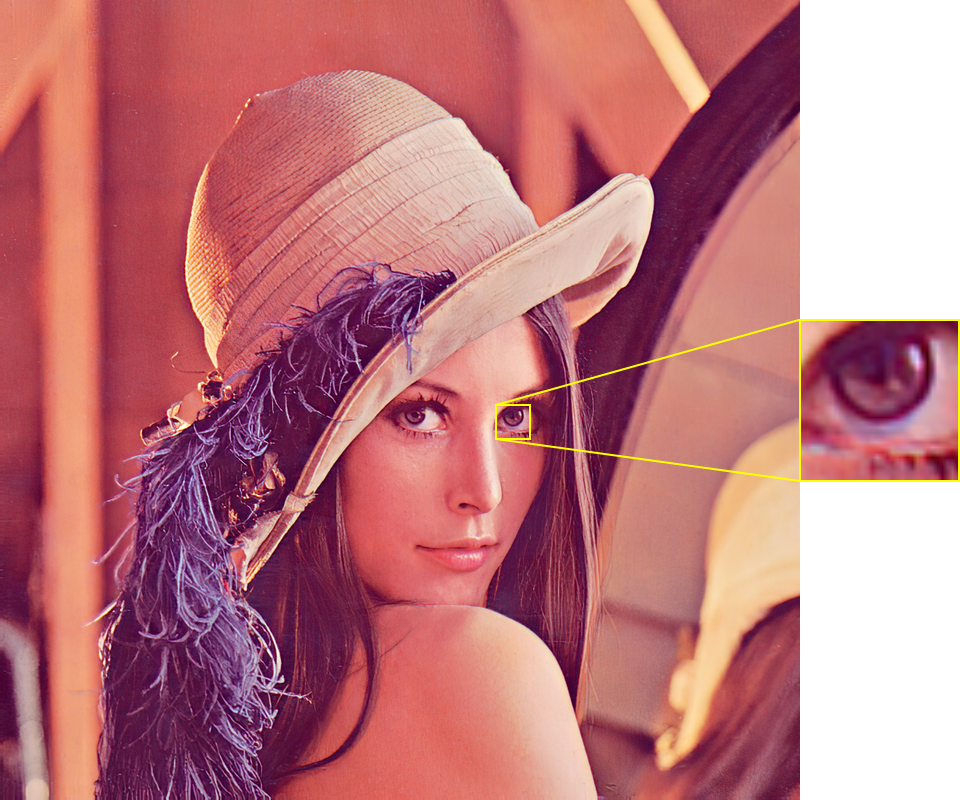
\includegraphics[width=\linewidth]{DCT/Lenna_eye.png}
    \caption{Выбираем область}
    \label{img:lenna-eye}
\end{figure}

%Для простоты будем использовать только синий канал изображения.
Сначала рассмотрим матрицу пикселей как двумерную дискретную функцию.
Расположим координаты так, чтобы в левом верхнем углу
располагался пиксель с координатами $p_{kj}, k = 0, j = 0$.
Визуализацию можно посмотреть на рисунке~\ref{img:pixels-dct}.

\begin{figure}[ht!]
    \centering
    \caption{Визуализация пикселей}
    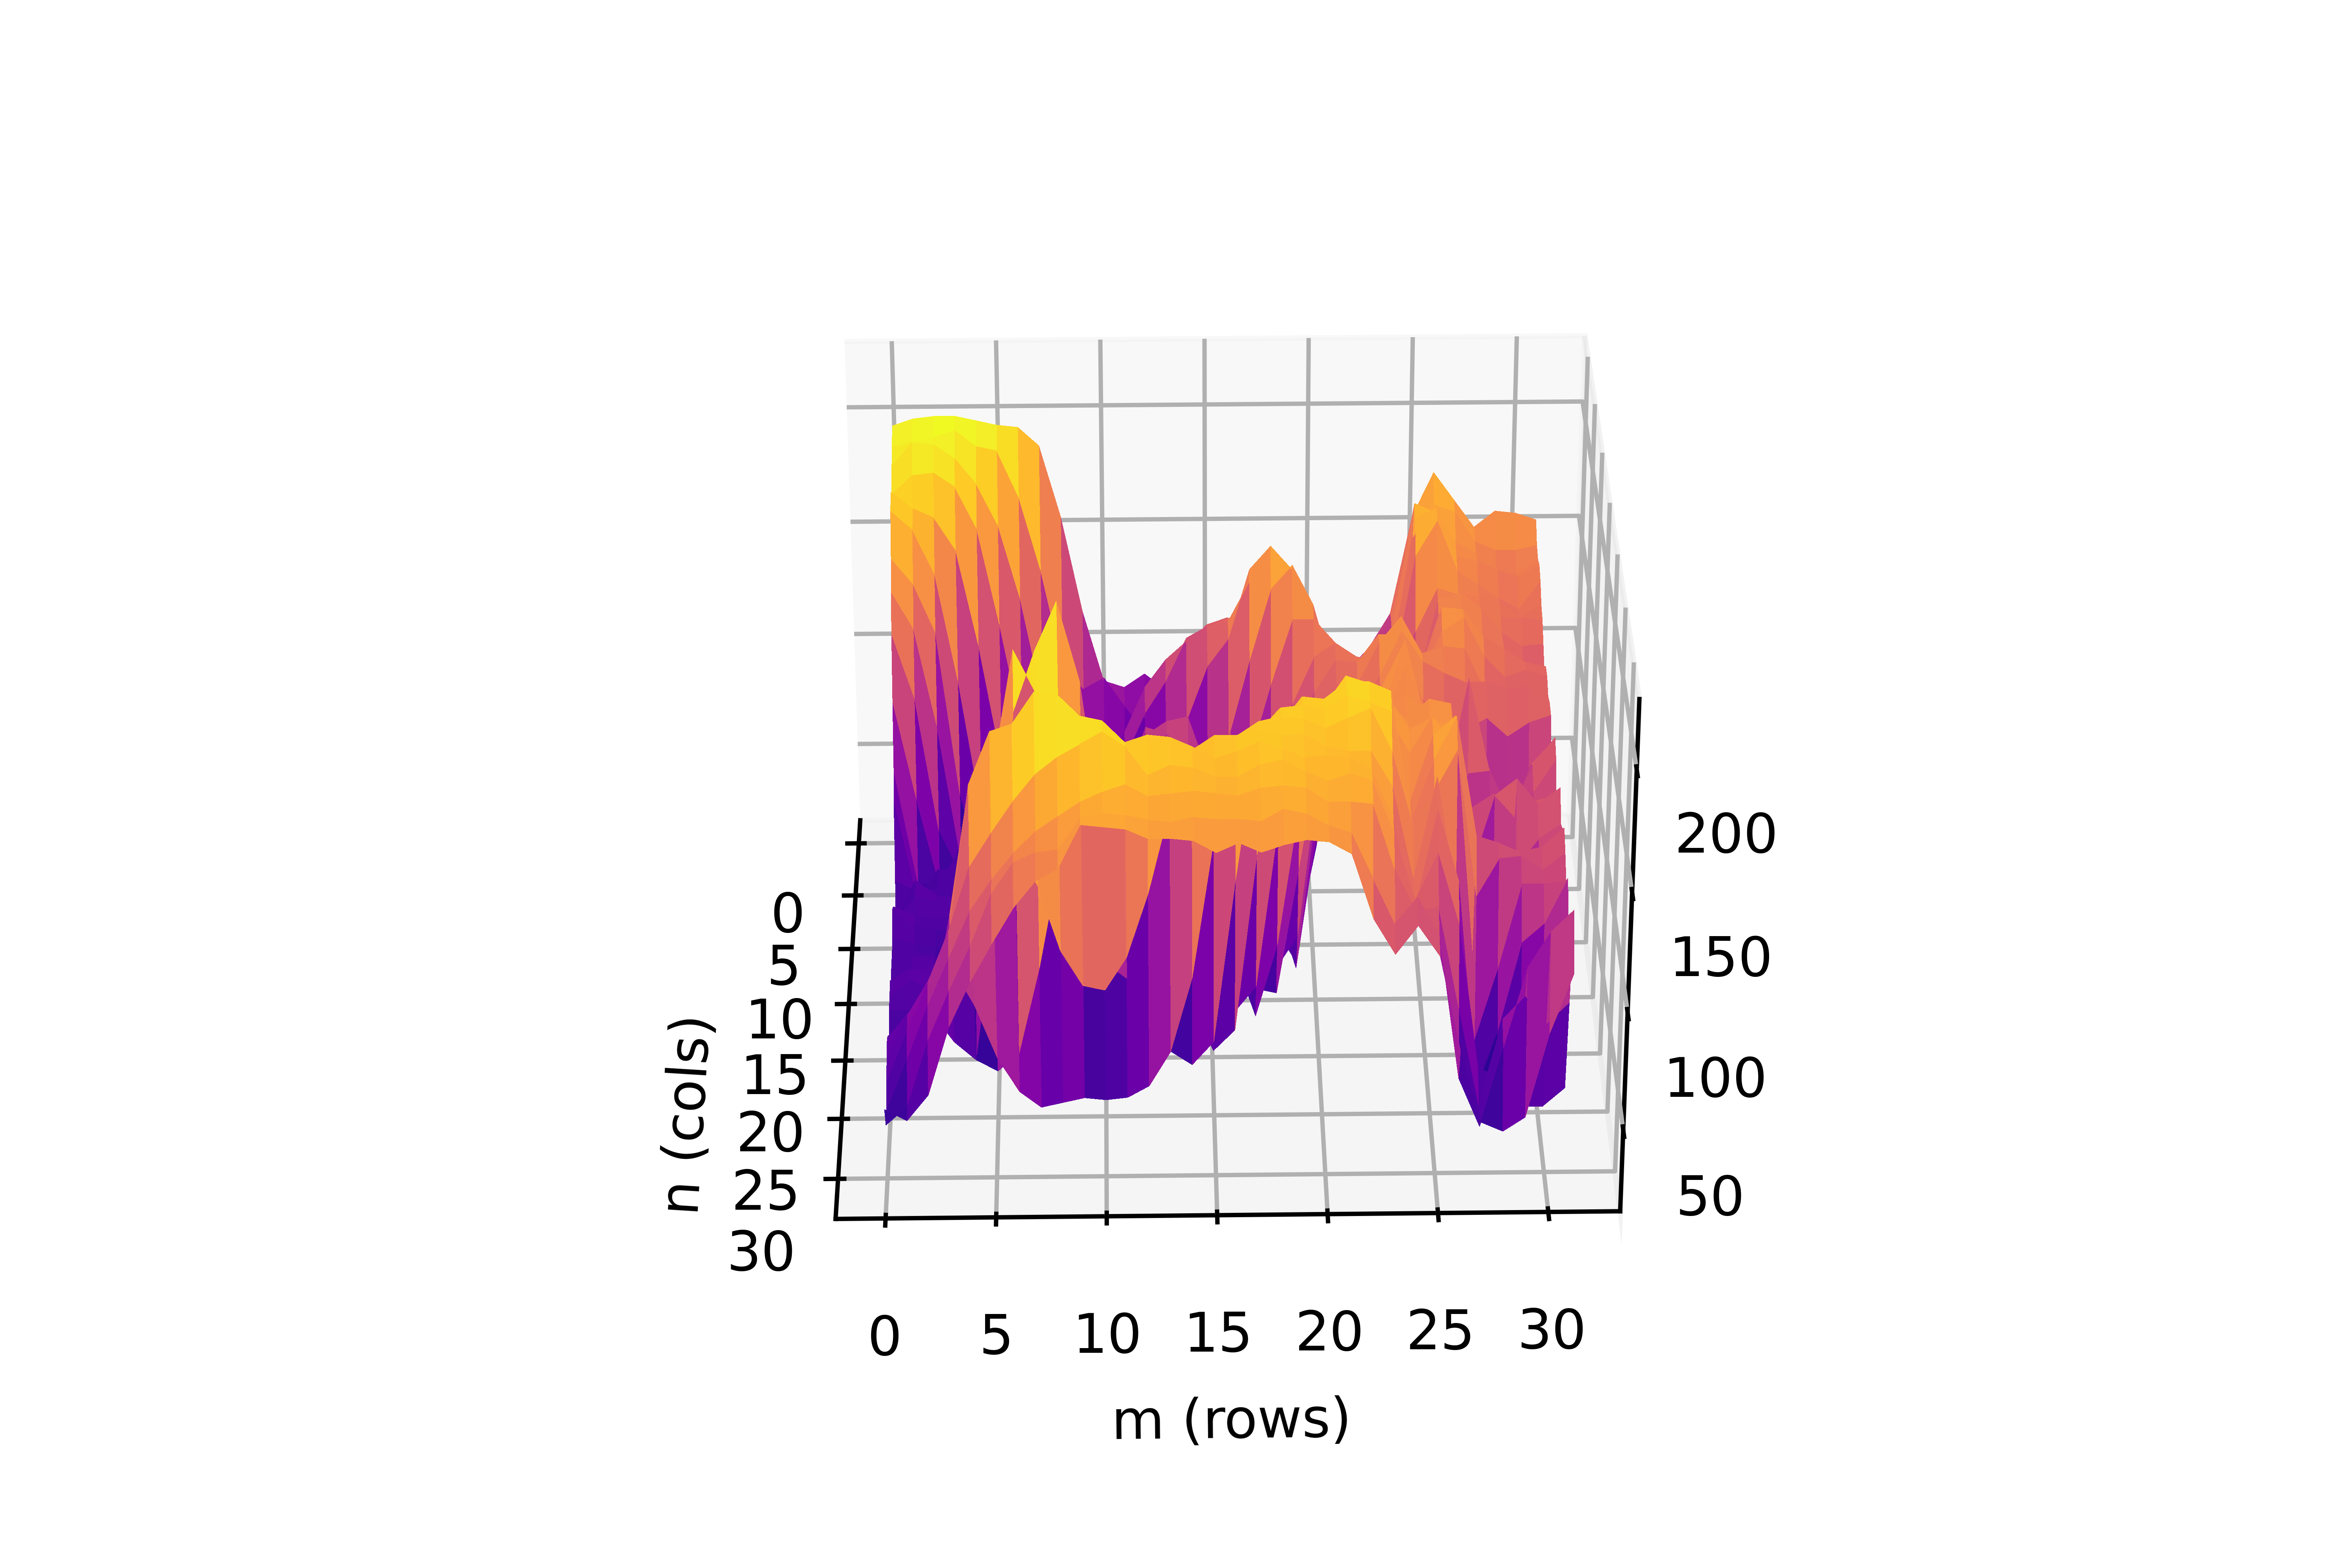
\includegraphics[width=\linewidth]{DCT/pixels.png}
    \label{img:pixels-dct}
\end{figure}

Умножим эту функцию справа на транспонированную матрицу ДКП
по формуле~\ref{eq:2d-matrix-dcp}. Мы получим новую функцию,
которая показана на рисунке~\ref{img:dct-1}.
Таким образом фактически ДКП применилось к каждой строке матрицы.
Из изображения видно, что наибольшие коэффициенты расположены
в нижней части спектра, то есть ближе к нулевому столбцу.

\begin{figure}[ht!]
    \centering
    \caption{После приминения ДКП к строкам матрицы}
    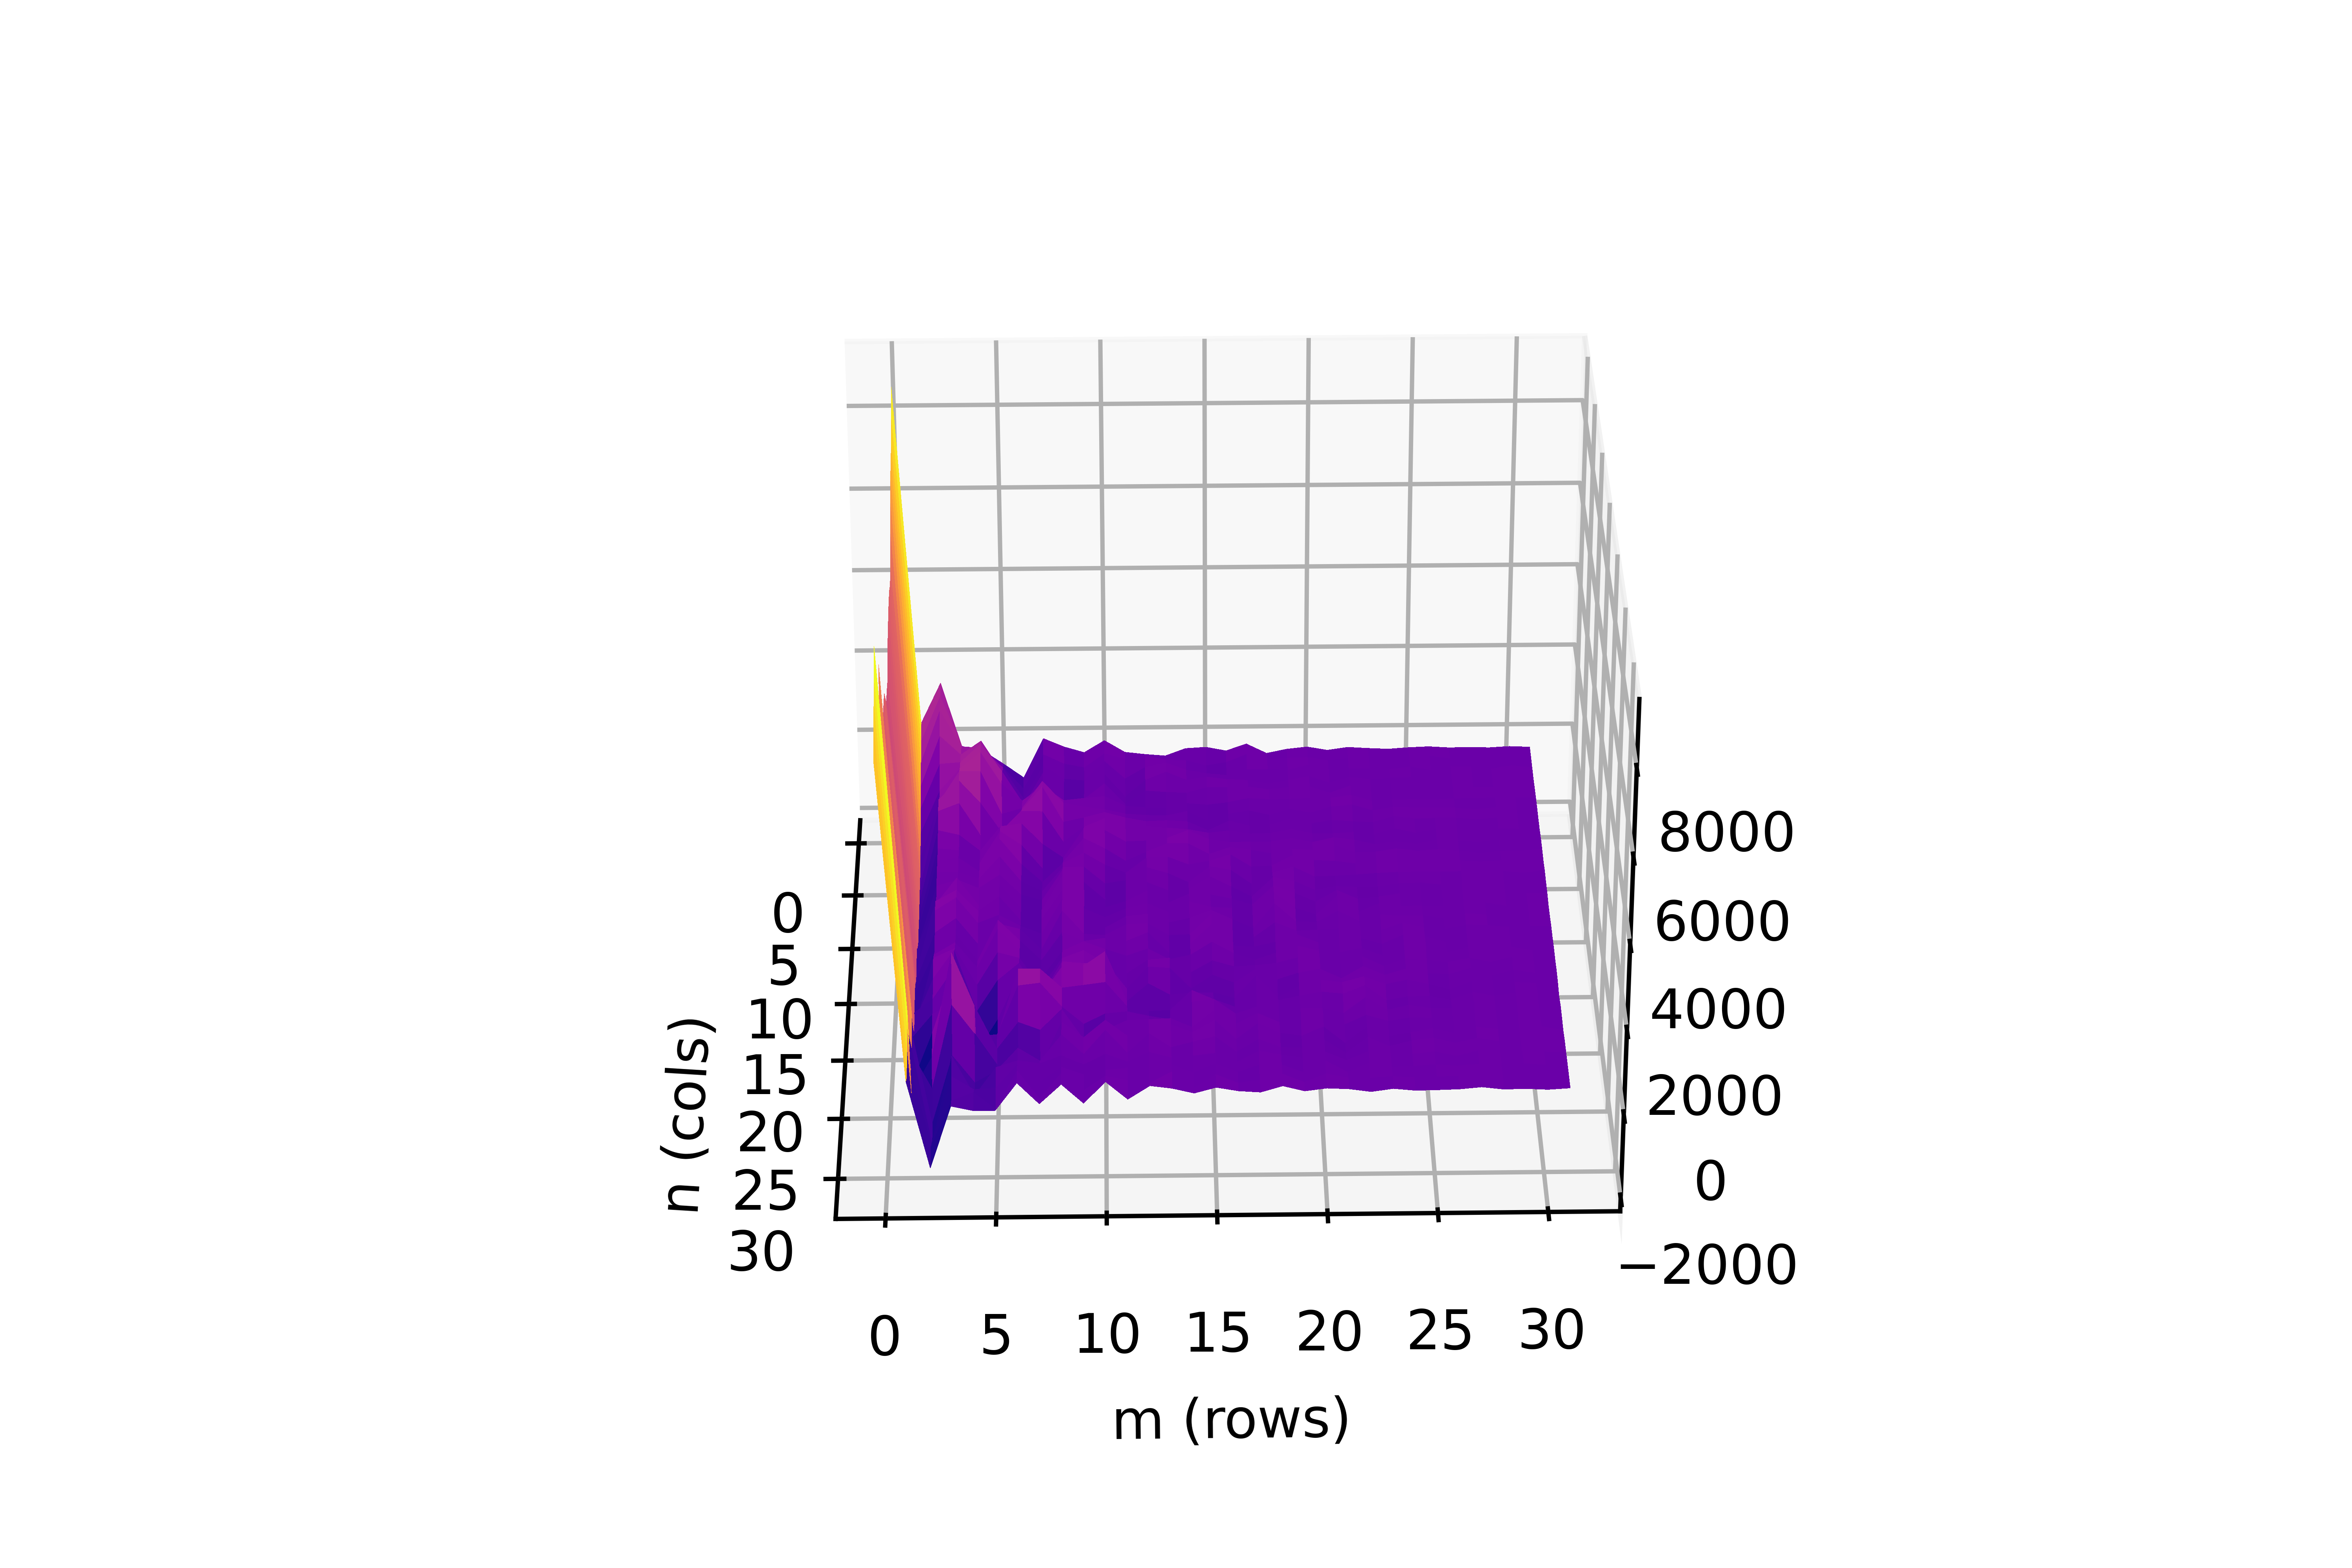
\includegraphics[width=\linewidth]{DCT/dct-1.png}
    \label{img:dct-1}
\end{figure}

К полученной матрице применим ДКП еще раз, в этот раз по столбцам.
В полученной матрице наибольшее значение имеет коэфициент с координатами
$k = 0, j = 0$. Этот коэффициент называется DC-коэффициент.
Остальные коэффициенты называются AC-коэффициентами.
Матрица показана на рисунке~\ref{img:dct-2}.

\begin{figure}[ht!]
    \centering
    \caption{После приминения ДКП к столбцам матрицы}
    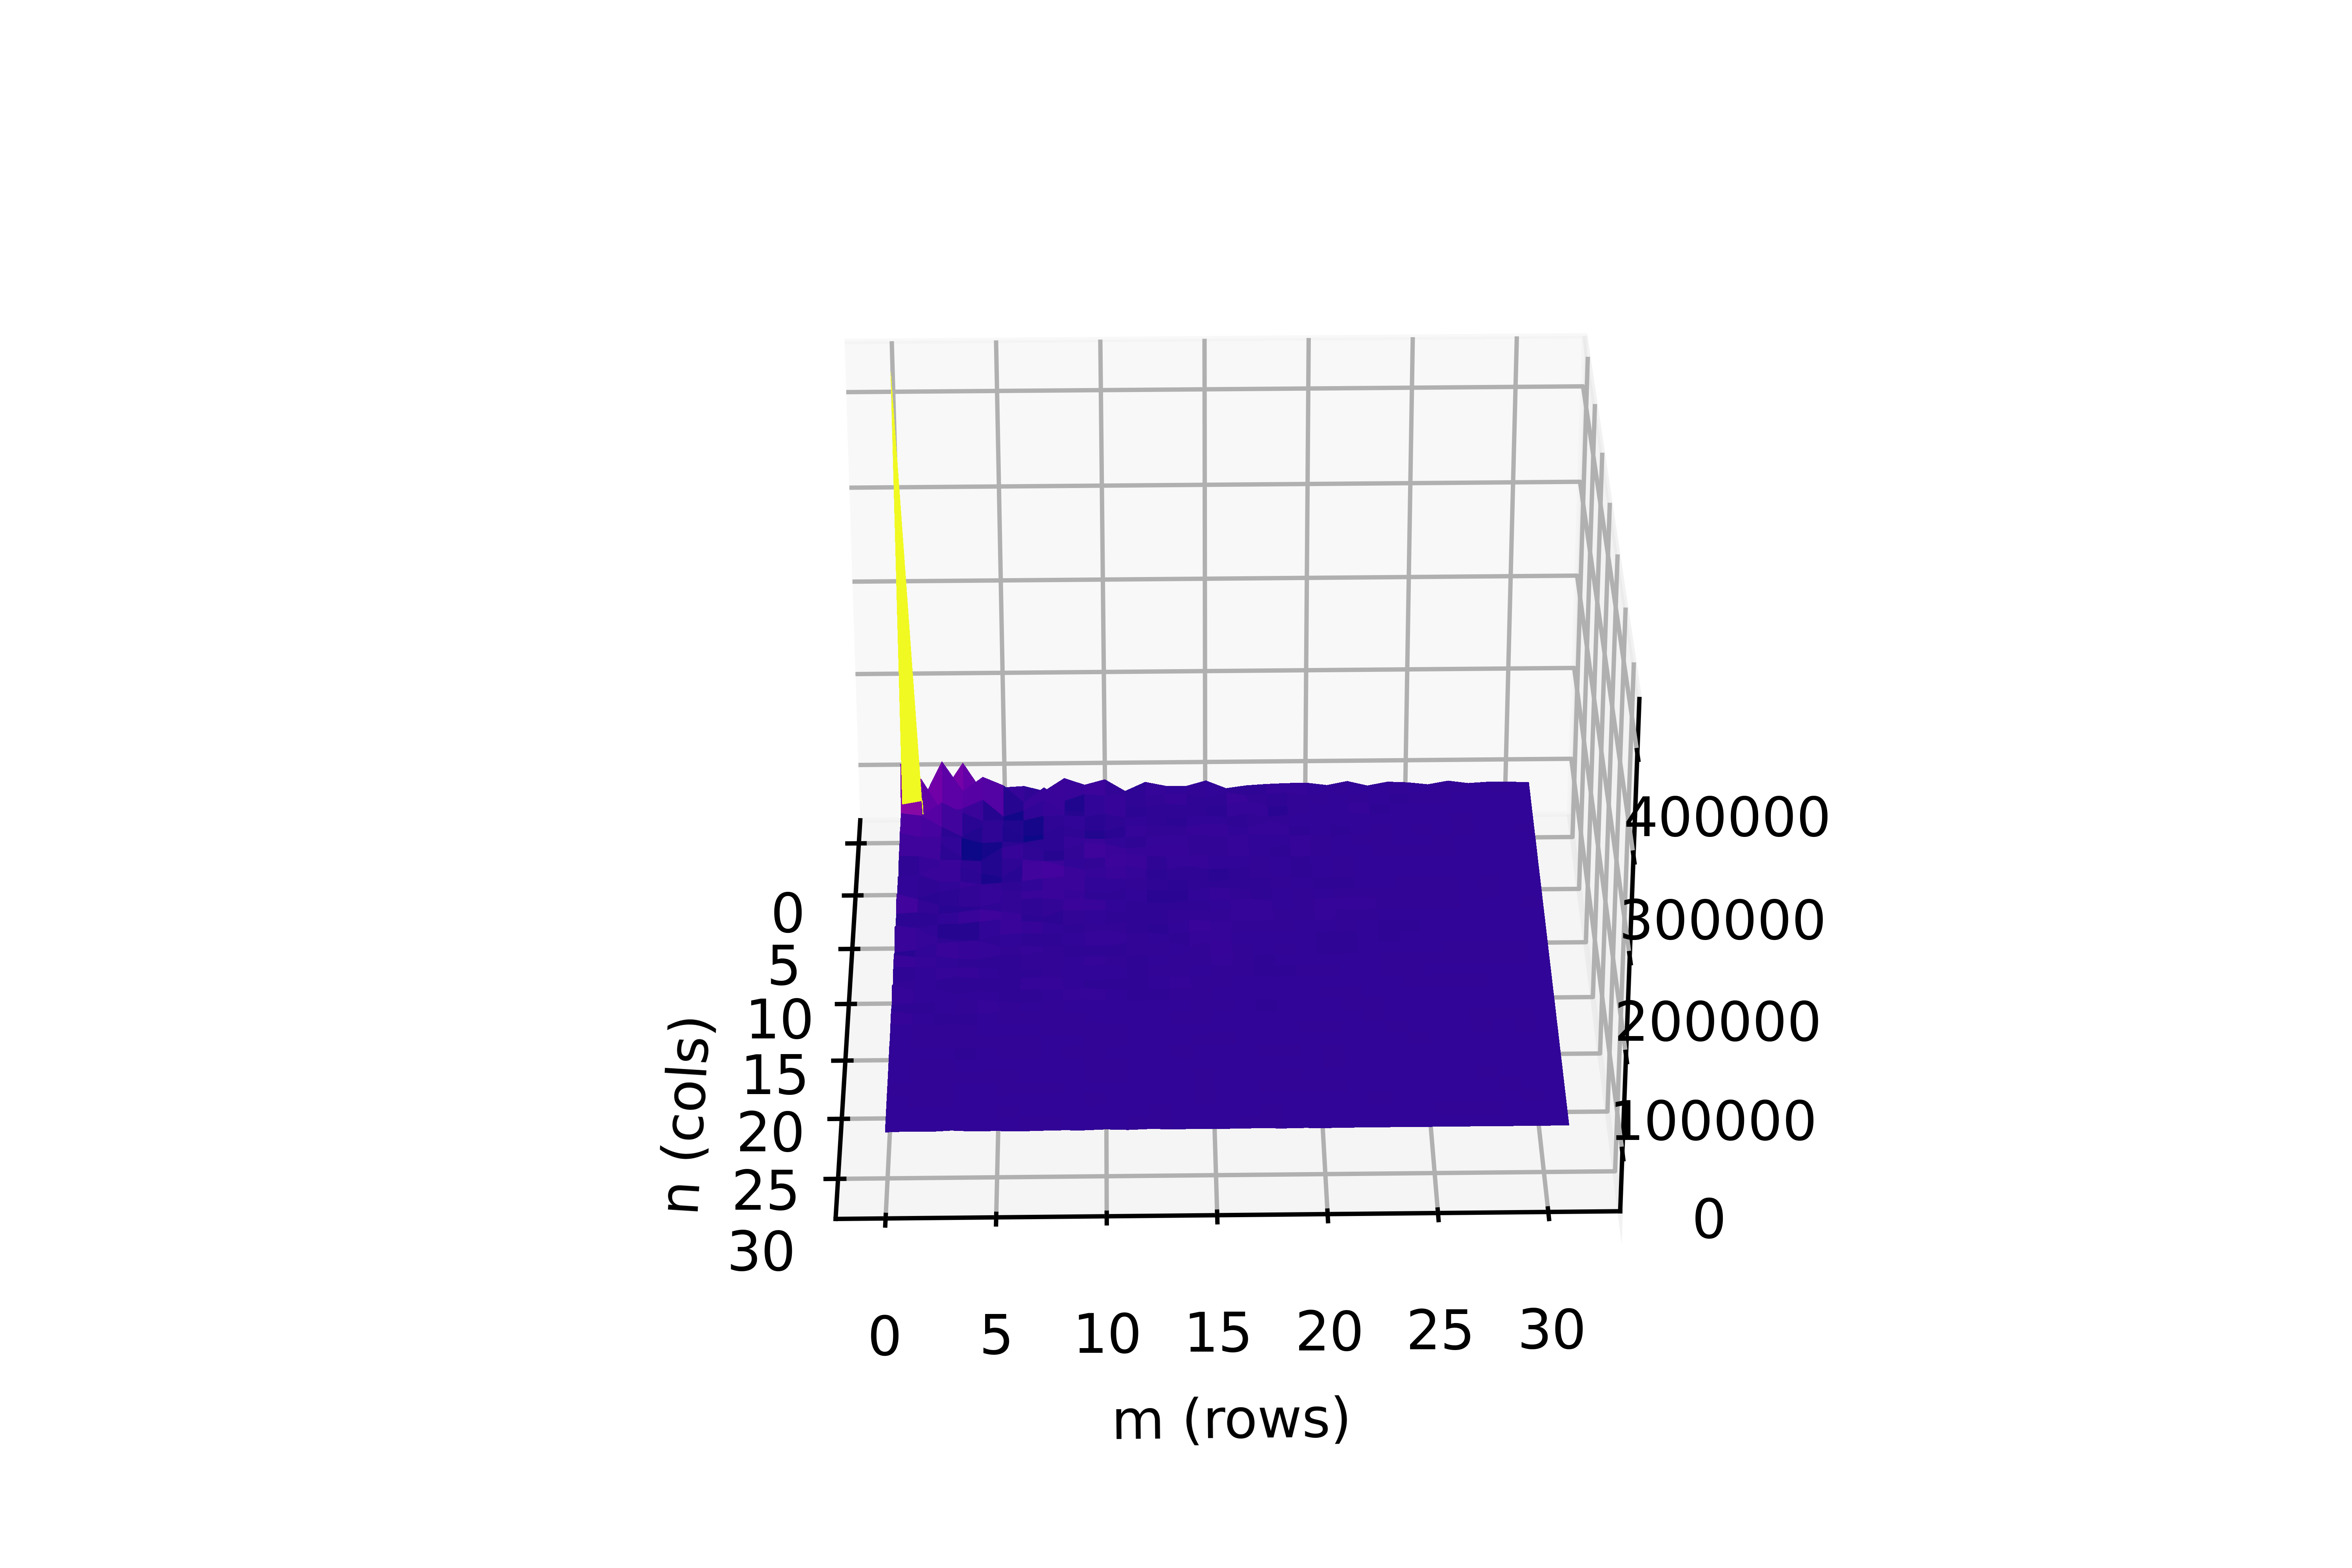
\includegraphics[width=\linewidth]{DCT/dct-2.png}
    \label{img:dct-2}
\end{figure}

DC-коэфициент блока равен среднему всех пикселей в блоке,
взятому с определенным коэффициентом. Удаляя все коэффициенты,
кроме DC, мы можем аппроксимировать блок пикселей их средним
арифметическим. Чем дальше коэффициент располагается от DC,
тем меньше психовизуальной информации он несет для человека,
и тем более незаметные детали изображения он хранит в себе.
Соответственно, основная идея алгоритма состоит в отбрасывании
наименее значимых коэффициентов. Это позволяет производить сжатие
изображения с потерями.

Алгоритм сжатия JPEG работает с каждым каналом отдельно, поэтому для
простоты рассмотрим работу JPEG на изображении в режиме градации серого.
В самом начале своей работы алгоритм разбивает изображение на блоки
8x8 пикселей. К каждому блоку применяется ДКП преобразование,
что равносильно разложению исходной матрицы по базису, состоящему
из 64 функций. Эти 64 функции показаны на рисунке~\ref{img:basis}.
Из этого рисунка видно, что помере отдаления от левого верхнего которая
функции становятся все более рельефными, что объясняет, почему они несут
наиболее мелкие детали изображения. Так же видно, что функция,
соответствующая DC-коэффициенту, представленая плоскостью. Очевидно,
что лучшим константным приближением функции
является ее математическое ожидание.
\begin{figure}[ht]
    \centering
    \caption{Базис ДКП}
    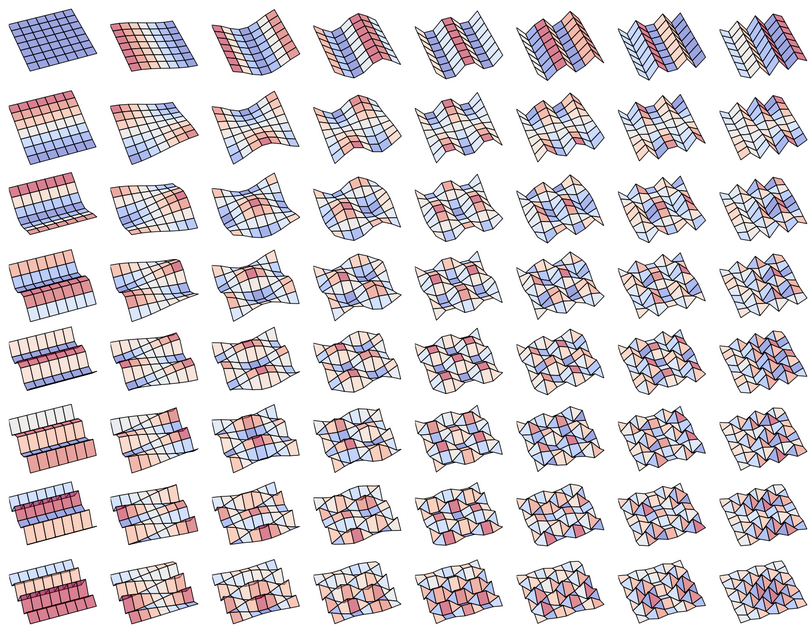
\includegraphics[width=.9\linewidth]{DCT/basis.png}
    \label{img:basis}
\end{figure}
После приминения ДКП преобразования к блоку матрице 8x8
получается другая матрица той же размерности. В соответствии с вышесказанным
эта матрица делится на области низких, средних и высоких частот. В таком порядке
убывает информативность коэффициентов. Это можно увидеть на рисунке~\ref{img:freq}.
\begin{figure}[ht]
    \centering
    \caption{Частотные области ДКП}
    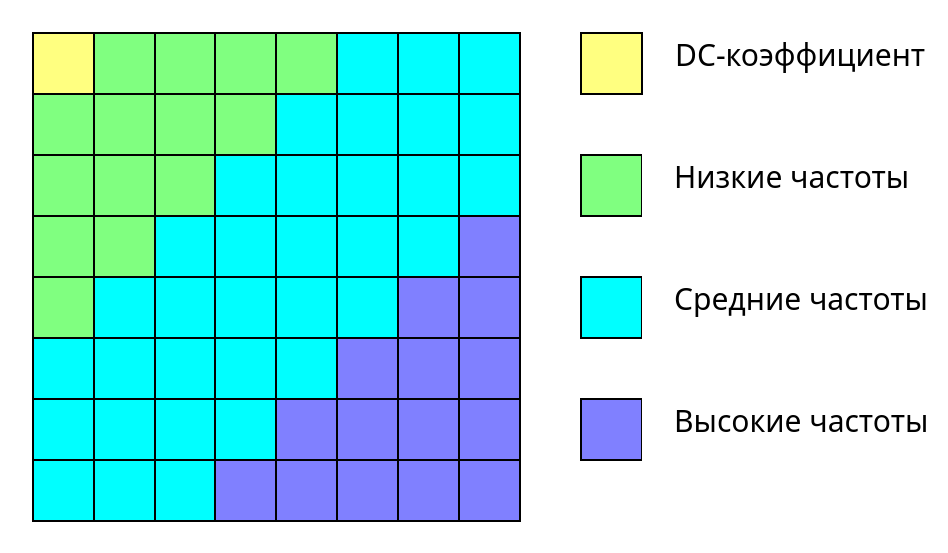
\includegraphics[width=.8\linewidth]{DCT/freq.png}
    \label{img:freq}
\end{figure}
Далее коэффициенты полученной ДКП матрицы квантуются.
Квантование происходит с приминением специальных матриц,
одна из таких матриц представлена в формуле~\ref{eq:q-matrix}.
\begin{equation} \label{eq:q-matrix}
Q=
\begin{bmatrix}
 16 & 11 & 10 & 16 & 24 & 40 & 51 & 61 \\
 12 & 12 & 14 & 19 & 26 & 58 & 60 & 55 \\
 14 & 13 & 16 & 24 & 40 & 57 & 69 & 56 \\
 14 & 17 & 22 & 29 & 51 & 87 & 80 & 62 \\
 18 & 22 & 37 & 56 & 68 & 109 & 103 & 77 \\
 24 & 35 & 55 & 64 & 81 & 104 & 113 & 92 \\
 49 & 64 & 78 & 87 & 103 & 121 & 120 & 101 \\
 72 & 92 & 95 & 98 & 112 & 100 & 103 & 99
\end{bmatrix}.
\end{equation}
Это матрица для 50\% качества, указанная в исходном стандарте JPEG.
Каждый элемент ДКП матрицы делится на коэффициент матрицы квантования,
стоящий в той же позиции. После этого результат округляется. В результате
этой операции обычно бывает так, что многие высокочастотные компоненты
округляются до нуля, а многие из остальных становятся небольшими положительными
или отрицательными числами, для представления которых требуется гораздно меньше бит.

При декодировании происходит обратный процесс --- матрица квантованных коэффициентов
почленное умножается на матрицу квантования, но из-за того, что до этого значения были округлены,
они восстанавливаются с некоторой погрешностью. Чем больше коэффициент квантования,
тем выше будет эта погрешность.

После квантования коэффициенты записываются в специальном зигзагообразном порядке,
показанном на рисунке~\ref{img:zigzag}. Таким образом коэффициенты упорядочиваются
от низких частот к высоким.
\begin{figure}[ht]
    \centering
    \caption{Зигзагообразный порядок}
    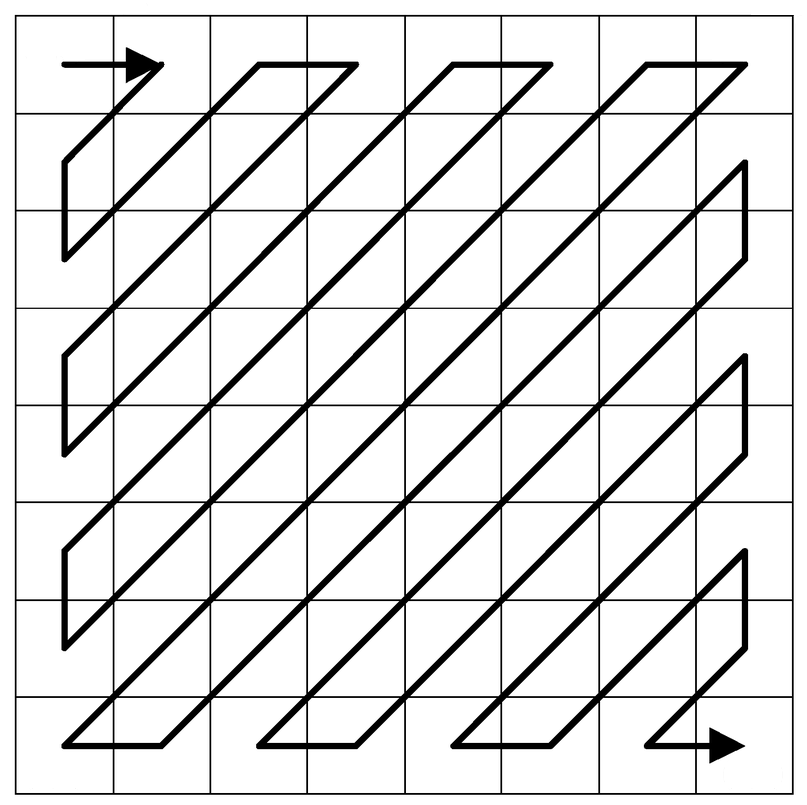
\includegraphics[width=.5\linewidth]{DCT/zigzag.png}
    \label{img:zigzag}
\end{figure}
После этого DC и AC коэффициенты кодируются отдельно.
Поскольку в изображениях часто встречаются
градиентные области, то DC коэффициенты соседних блоков
скорелированны, поэтому первым этапом их кодирования
становится дифференциальная импульсно-кодовая модуляция (ДИКМ).
То есть кодируются не сами коэффициенты, а разница между двумя
соседними коэффициентами.
AC коэффициенты кодируются с помощью кодирования длин серий (КДС).
То есть повторяющиеся символы заменяются на символ и количество его повторов.
После этого к DC и AC коэффициентам применяется энтропийное кодирование с помощью
алгоритма Хаффмана.

Мы разобрали работу алгоритма для одноканального изображения.
В RGB изображениях такой алгоритм применяется к каждому каналу отдельно.
Так же часто кодированию предшествует дополнительный этап,
на котором RGB преобразуется в цветовое пространство
YC\textsubscript{B}C\textsubscript{R}.
Дело в том, что человеческий глаз более чувствителен к перепадам
яркости, чем к перепаду цвета.
В YC\textsubscript{B}C\textsubscript{R} первый канал Y отвечает за яркость,
C\textsubscript{B} и C\textsubscript{R} отвечают за синию и красную компоненты.
После преобразования в YC\textsubscript{B}C\textsubscript{R}
над C\textsubscript{B} и C\textsubscript{R} производится субдискретизация:
каналы разбиваются на небольшие блоки и значения пикселей в этих блоках усредняются.
Таким образом разрешение в этих каналах понижается еще сильнее
и изображение сжимается еще сильнее.
Вся схема алгоритма представлена на рисунке~\ref{img:jpeg-alg}
\begin{figure}[ht]
    \centering
    \caption{Схематичное изображение JPEG}
    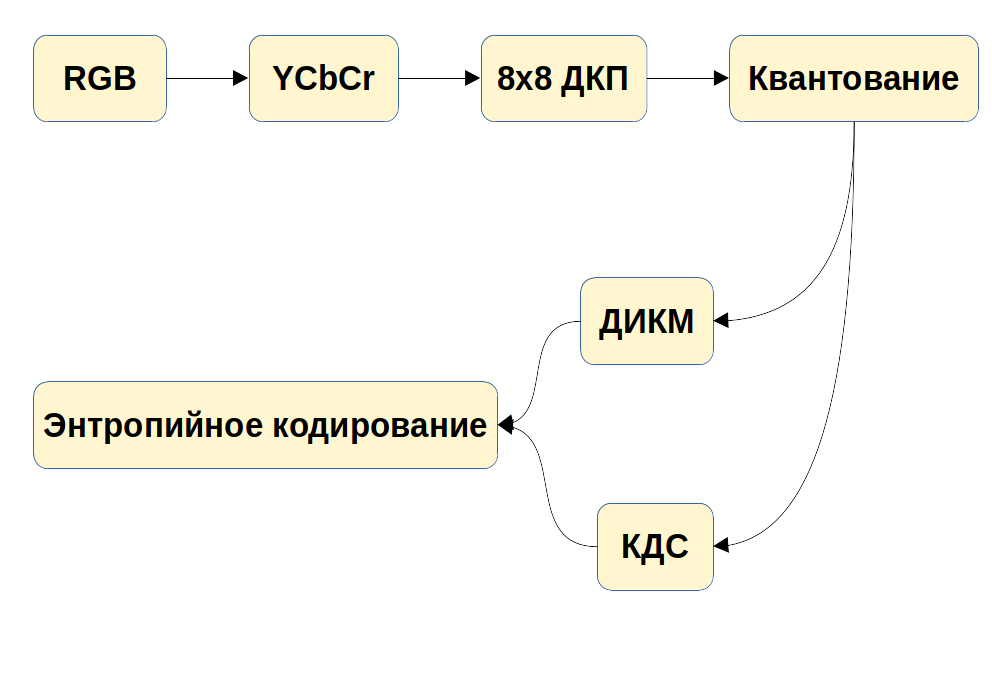
\includegraphics[width=.8\linewidth]{DCT/jpeg-alg.png}
    \label{img:jpeg-alg}
\end{figure}

\section{JSteg}
JSteg --- стеганографический алгоритм, работающий с JPEG файлами.
JSteg во многом опирается на работу кодировщика JPEG. Алгоритмы
кодирования и декодирования JPEG абсолютно симметричны.
JSteg вмешиваетсяв в работу декодировщика, а именно прерывает
его на этапе умножения ДКП коэффициентов на матрицу квантования.
После этого JSteg записывает в упорядоченные зигзагообразным образом
ДКП коэффициенты кодируемую информацию методом LSB. После этого вызывается
кодировщик, который записывает измененные ДКП коэффициенты обратно в JPEG
изображение.

Рассмотрим достоинства и недостатки этого метода.
К доистоинствам можно отнести следующее:
\begin{enumerate}
    \item Низкая вычислительная сложность.
    \item Алгоритм обеспечивает большую вместимость стегосообщений:
    стегосообщение может занимать до 13\% объема контейнера.
    \item Изменения, вносимые в контейнер, незаметны для человеческого глаза.
\end{enumerate}
Но у метода так же есть и существенные недостатки:
\begin{enumerate}
    \item Метод неустойчив к квантованию ДКП коэффициентов.
    Как уже говорилось ранее, операция квантования
    восстанавливает и сохраняет коэффициент с некоторой погрешностью,
    поэтому если открыть в редакторе стегоконтейнер, в котором
    содержится сообщение, закодированное методом JSteg,
    то после пересохранения этого файла сообщение полностью уничтожится. 
    \item Из предыдущих соображения становится ясно, что метод не устойчив
    к сжатию. Это так же обусловлено еще и тем, что при сжатии коэффициенты
    квантования увеличиваются, а значит часть ДКП коэффициентов обнулится,
    а у другой части погрешность восстановления станет еще больше.
\end{enumerate}
Рассмотрим реализацию метода на Python. Код приведен в листинге~\ref{code:jsteg}.
По сути метод представляет собой LSB, только вместо пространственной области
используется спектральная. В данном случае наименее значимый бит меняется
у коэффициентов ДКП изображения, упорядоченных зигзагообразным способом. 
\lstinputlisting[language=Python, label={code:jsteg}, style=simplecode, caption=Реализация JSteg, frame=single]{Code/jsteg.py}

\section{Метод относительной замены величин коэффициентов ДКП}
Этот метод использует идеи, схожие с методами расширения спектра, а именно:
вместо того, чтобы кодировать 1 бит информации в одном коэффициенте ДКП,
метод предлагает кодировать 1 бит информации за счет нескольких коэффициентов ДКП.
Этого можно добиться, кодируя информацию за счет изменения разности между
набором различных коэффициентов ДКП.

Алгоритм Коха-Жао использует 2 коэффициента ДКП.
Формальное описание приводится в алгоритме~\ref{alg:koch-jao}.
Алгоритм декодирования строится симметрично.
Это простейший метод из данного семейства. К доистоинствам
метода можно отнести то, что он устойчив к квантованию ДКП-коэффициентов
и сжатию. Особенно если применять его в паре с помехоустойчив кодироавнием.
Но у метода так же есть и серьезные недостатки:
\begin{enumerate}
    \item Метод вносит заметные искажения в контейнер.
    \item Метод легко детектируется.
\end{enumerate}

\begin{algorithm}[ht!]
    \KwData{Контейнер, Сообщение}
    \KwResult{Заполненный стегоконтейнер}
     $N \leftarrow$ Длина сообщения в битах\;
     $Message \leftarrow$ Бинарное представление сообщения\;
     $DCT$-$blocks \leftarrow$ Массив из блоков ДКП контейнера\;
     $k, l \leftarrow$ Позиция коэффициента ДКП из низкой полосы частот\;
     \For{$i = 1, 2, \ldots, N$}{
         \eIf{$Message[i] = 0$}{
             Сделать $|DCT$-$blocks[i][k][l] - DCT$-$blocks[i][k][l]| < 25$\;
         }{
             Сделать $|DCT$-$blocks[i][k][l] - DCT$-$blocks[i][k][l]| > 25$\;
         }
     }
     $Container \leftarrow$ Новый контейнер, полученный из обратного преобразования ДКП-блоков\;
     \caption{Алгоритм Коха-Жао}
    \label{alg:koch-jao}
\end{algorithm}

Модифицированной версией этого метода является метод Бенгама-Мемона-Эо-Юнга.
Модификации подверглись два направления:
\begin{enumerate}
    \item Встраивание происходит только в наиболее подходящие ДКП-блоки.
    \item Используются не 2, а 3 коэффициента ДКП. Это существенно снижает
    вносимые в контейнер искажения.
\end{enumerate}.
Рассмотрим каждую модификацию в отдельности.

Наиболее подходящие коэффициенты выбираются по следующим признакам:
\begin{enumerate}
    \item Блок не должен иметь слишком резких переходов яркости.
    \item Блок не должен быть слишком монотонным.
\end{enumerate}
Для оценки этих параметров вводится два коэффициента: P\textsubscript{L} и P\textsubscript{H}.
Превышение первого коэффициента или недостижение второго будет указывать на то,
что блок не пригоден для встраивания. Для получения первой оценки нужно проссумировать модуляция
низкочастотных коэффициентов, а для получения второй оценки нужно проссумировать модули высокочастотных
коэффициентов.

Само встраивание происходит в два этапа.
На первом этапе выбираются три коэффициента из низкой полосы частот.
Для обеспечения большой стойкости они могут выбираться псевдослучайно.
На втором этапе коэффициенты модифицируются. Если кодируется 0,
то третий коэффициент должен стать больше первых двух, а если 1,
то третий коэффициент должен стать меньше, соответственно.
После встраивания запоминаются номера блоков, в которых закодирована информация.
Декодирование происходит симметричным образом с той лишь разницей,
что вместо поиска подходящих блоков используются запомненные на прыдедущем этапе блоки.
Реализацию метода на Python можно найти в приложении~\ref{appendix-a}.

\backmatter %% Здесь заканчивается нумерованная часть документа и начинаются ссылки

\appendix   % Тут идут приложения

\end{document}